\begin{cverbatim}
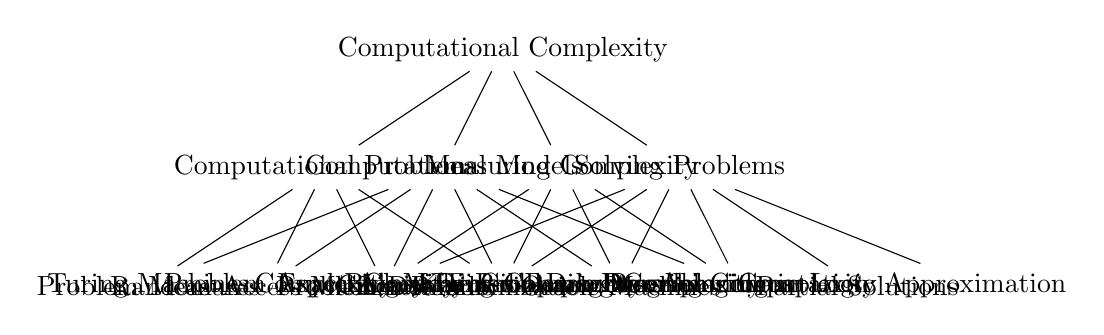
\begin{tikzpicture}
\node {Computational Complexity} % root
    child { node {Computational Problems}
                child { node {Problem Measures} }
                child { node {Problem Aspects} }
                child { node {Problem Domains} }
                child { node {Key Problems} }
    }
    child { node {Computational Models}
                child { node {Turing Machines} }
                child { node {Random-Access Machines} }
                child { node {Circuits} }
                child { node {Binary Decision Diagrams} }
                child { node {Oracle Machines} }
                child { node {Programming in Logic} }
    }
    child { node {Measuring Complexity}
                child { node {Complexity Measures} }
                child { node {Classifying Complexity} }
                child { node {Comparing Complexity} }
                child { node {Describing Complexity} }
    }
    child { node {Solving Problems}
                child { node {Exact Algorithms} }
                child { node {Randomization} }
                child { node {Fixed-Parameter Algorithms} }
                child { node {Parallel Computation} }
                child { node {Partial Solutions} }
                child { node {Approximation} }
};
\end{tikzpicture}
\end{cverbatim}

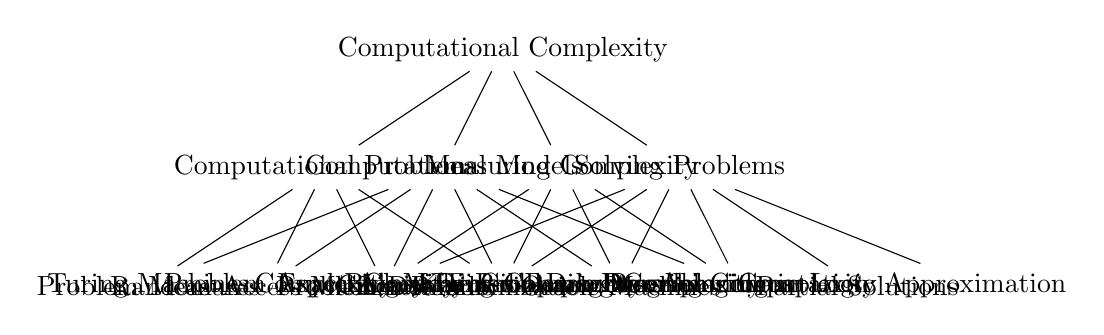
\begin{tikzpicture}
\node {Computational Complexity} % root
    child { node {Computational Problems}
                child { node {Problem Measures} }
                child { node {Problem Aspects} }
                child { node {Problem Domains} }
                child { node {Key Problems} }
    }
    child { node {Computational Models}
                child { node {Turing Machines} }
                child { node {Random-Access Machines} }
                child { node {Circuits} }
                child { node {Binary Decision Diagrams} }
                child { node {Oracle Machines} }
                child { node {Programming in Logic} }
    }
    child { node {Measuring Complexity}
                child { node {Complexity Measures} }
                child { node {Classifying Complexity} }
                child { node {Comparing Complexity} }
                child { node {Describing Complexity} }
    }
    child { node {Solving Problems}
                child { node {Exact Algorithms} }
                child { node {Randomization} }
                child { node {Fixed-Parameter Algorithms} }
                child { node {Parallel Computation} }
                child { node {Partial Solutions} }
                child { node {Approximation} }
};
\end{tikzpicture}

\begin{cverbatim}
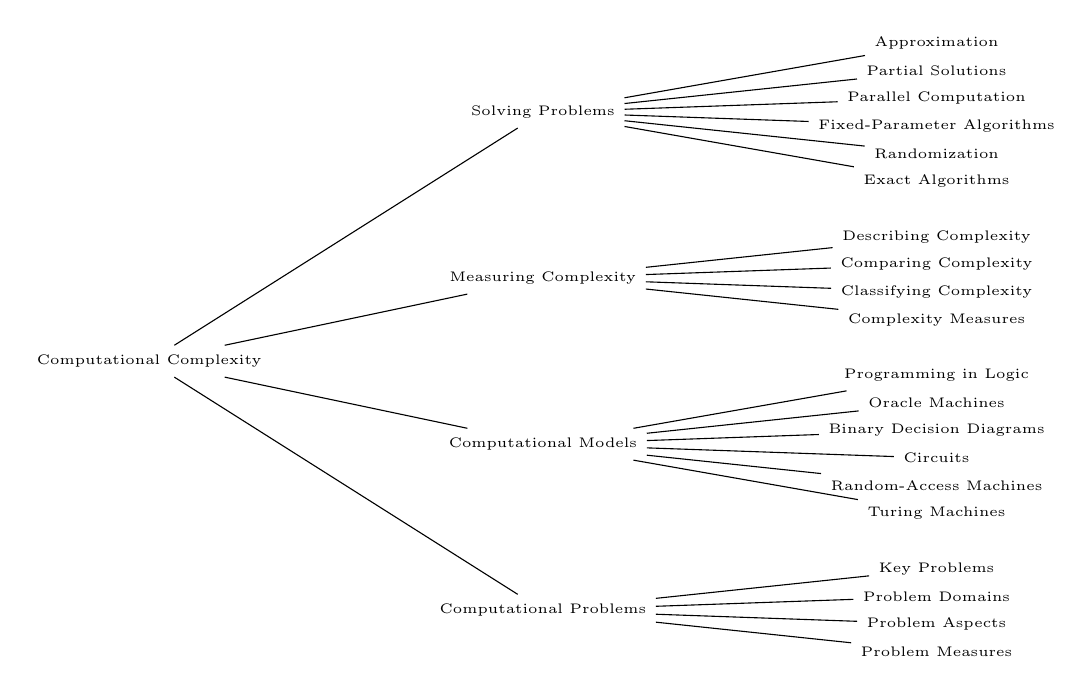
\begin{tikzpicture}[font=\tiny,
                    grow=right, level 1/.style={sibling distance=6em},
                                level 2/.style={sibling distance=1em}, level distance=5cm]
\node {Computational Complexity} % root
    child { node {Computational Problems}
                child { node {Problem Measures} }
                child { node {Problem Aspects} }
                child { node {Problem Domains} }
                child { node {Key Problems} }
    }
    child { node {Computational Models}
                child { node {Turing Machines} }
                child { node {Random-Access Machines} }
                child { node {Circuits} }
                child { node {Binary Decision Diagrams} }
                child { node {Oracle Machines} }
                child { node {Programming in Logic} }
    }
    child { node {Measuring Complexity}
                child { node {Complexity Measures} }
                child { node {Classifying Complexity} }
                child { node {Comparing Complexity} }
                child { node {Describing Complexity} }
    }
    child { node {Solving Problems}
                child { node {Exact Algorithms} }
                child { node {Randomization} }
                child { node {Fixed-Parameter Algorithms} }
                child { node {Parallel Computation} }
                child { node {Partial Solutions} }
                child { node {Approximation} }
};
\end{tikzpicture}
\end{cverbatim}

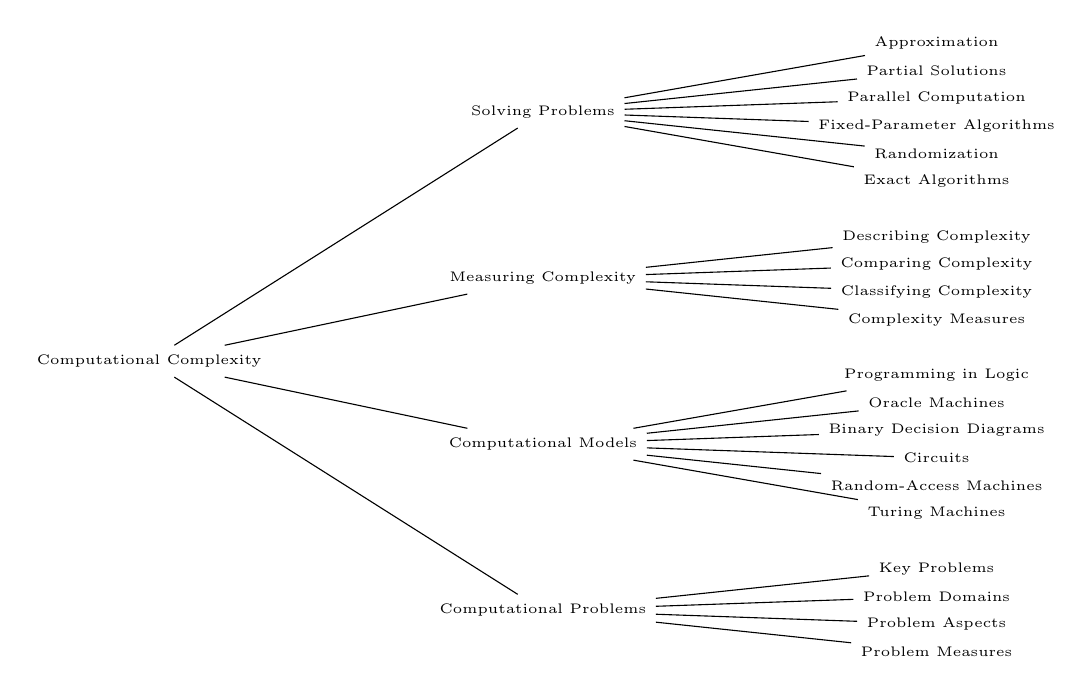
\begin{tikzpicture}[font=\tiny,
                    grow=right, level 1/.style={sibling distance=6em},
                                level 2/.style={sibling distance=1em}, level distance=5cm]
\node {Computational Complexity} % root
    child { node {Computational Problems}
                child { node {Problem Measures} }
                child { node {Problem Aspects} }
                child { node {Problem Domains} }
                child { node {Key Problems} }
    }
    child { node {Computational Models}
                child { node {Turing Machines} }
                child { node {Random-Access Machines} }
                child { node {Circuits} }
                child { node {Binary Decision Diagrams} }
                child { node {Oracle Machines} }
                child { node {Programming in Logic} }
    }
    child { node {Measuring Complexity}
                child { node {Complexity Measures} }
                child { node {Classifying Complexity} }
                child { node {Comparing Complexity} }
                child { node {Describing Complexity} }
    }
    child { node {Solving Problems}
                child { node {Exact Algorithms} }
                child { node {Randomization} }
                child { node {Fixed-Parameter Algorithms} }
                child { node {Parallel Computation} }
                child { node {Partial Solutions} }
                child { node {Approximation} }
};
\end{tikzpicture}

\begin{cverbatim}
\begin{tikzpicture}[font=\footnotesize, text width=2.7cm, align=flush center,
                    grow cyclic, 
                    level 1/.style={level distance=2.5cm, sibling angle=90},
                    level 2/.style={text width=2cm, font=\tiny, level distance=3cm, sibling angle=30}]
\node[font=\normalsize\bfseries] {\hskip0pt Computational Complexity} % root
    child { node {Computational Problems}
                child { node {Problem Measures} }
                child { node {Problem Aspects} }
                child { node {Problem Domains} }
                child { node {Key Problems} }
    }
    child { node {Computational Models}
                child { node {Turing Machines} }
                child { node {Random-Access Machines} }
                child { node {Circuits} }
                child { node {Binary Decision Diagrams} }
                child { node {Oracle Machines} }
                child { node {Programming in Logic} }
    }
    child { node {Measuring Complexity}
                child { node {Complexity Measures} }
                child { node {Classifying Complexity} }
                child { node {Comparing Complexity} }
                child { node {Describing Complexity} }
    }
    child { node {Solving Problems}
                child { node {Exact Algorithms} }
                child { node {Randomization} }
                child { node {Fixed-Parameter Algorithms} }
                child { node {Parallel Computation} }
                child { node {Partial Solutions} }
                child { node {Approximation} }
};
\end{tikzpicture}
\end{cverbatim}

\begin{tikzpicture}[font=\footnotesize, text width=2.7cm, align=flush center,
                    grow cyclic, 
                    level 1/.style={level distance=2.5cm, sibling angle=90},
                    level 2/.style={text width=2cm, font=\tiny, level distance=3cm, sibling angle=30}]
\node[font=\normalsize\bfseries] {\hskip0pt Computational Complexity} % root
    child { node {Computational Problems}
                child { node {Problem Measures} }
                child { node {Problem Aspects} }
                child { node {Problem Domains} }
                child { node {Key Problems} }
    }
    child { node {Computational Models}
                child { node {Turing Machines} }
                child { node {Random-Access Machines} }
                child { node {Circuits} }
                child { node {Binary Decision Diagrams} }
                child { node {Oracle Machines} }
                child { node {Programming in Logic} }
    }
    child { node {Measuring Complexity}
                child { node {Complexity Measures} }
                child { node {Classifying Complexity} }
                child { node {Comparing Complexity} }
                child { node {Describing Complexity} }
    }
    child { node {Solving Problems}
                child { node {Exact Algorithms} }
                child { node {Randomization} }
                child { node {Fixed-Parameter Algorithms} }
                child { node {Parallel Computation} }
                child { node {Partial Solutions} }
                child { node {Approximation} }
};
\end{tikzpicture}

\begin{cverbatim}
\begin{tikzpicture}[mindmap, every node/.style={concept, execute at begin node=\hskip0pt}, % execute ... is to get rid of overfullbox warning
                    concept color=black!20,
                    grow cyclic, 
                    level 1/.append style={level distance=4.5cm, sibling angle=90},
                    level 2/.append style={level distance=3cm, sibling angle=45}]
\node[root concept] {Computational Complexity} % root
    child { node {Computational Problems}
                child { node {Problem Measures} }
                child { node {Problem Aspects} }
                child { node {Problem Domains} }
                child { node {Key Problems} }
    }
    child { node {Computational Models}
                child { node {Turing Machines} }
                child { node {Random-Access Machines} }
                child { node {Circuits} }
                child { node {Binary Decision Diagrams} }
                child { node {Oracle Machines} }
                child { node {Programming in Logic} }
    }
    child { node {Measuring Complexity}
                child { node {Complexity Measures} }
                child { node {Classifying Complexity} }
                child { node {Comparing Complexity} }
                child { node {Describing Complexity} }
    }
    child { node {Solving Problems}
                child { node {Exact Algorithms} }
                child { node {Randomization} }
                child { node {Fixed-Parameter Algorithms} }
                child { node {Parallel Computation} }
                child { node {Partial Solutions} }
                child { node {Approximation} }
};
\end{tikzpicture}
\end{cverbatim}

\begin{tikzpicture}[mindmap, every node/.style={concept, execute at begin node=\hskip0pt}, % execute ... is to get rid of overfullbox warning
                    concept color=black!20,
                    grow cyclic, 
                    level 1/.append style={level distance=4.5cm, sibling angle=90},
                    level 2/.append style={level distance=3cm, sibling angle=45}]
\node[root concept] {Computational Complexity} % root
    child { node {Computational Problems}
                child { node {Problem Measures} }
                child { node {Problem Aspects} }
                child { node {Problem Domains} }
                child { node {Key Problems} }
    }
    child { node {Computational Models}
                child { node {Turing Machines} }
                child { node {Random-Access Machines} }
                child { node {Circuits} }
                child { node {Binary Decision Diagrams} }
                child { node {Oracle Machines} }
                child { node {Programming in Logic} }
    }
    child { node {Measuring Complexity}
                child { node {Complexity Measures} }
                child { node {Classifying Complexity} }
                child { node {Comparing Complexity} }
                child { node {Describing Complexity} }
    }
    child { node {Solving Problems}
                child { node {Exact Algorithms} }
                child { node {Randomization} }
                child { node {Fixed-Parameter Algorithms} }
                child { node {Parallel Computation} }
                child { node {Partial Solutions} }
                child { node {Approximation} }
};
\end{tikzpicture}

\begin{cverbatim}
\begin{tikzpicture}
        [mindmap, 
         every node/.style={concept, execute at begin node=\hskip0pt},
         root concept/.append style={
           concept color=black, fill=white, line width=1ex, text=black},
         text=white,
         grow cyclic, 
         level 1/.append style={level distance=4.5cm, sibling angle=90},
         level 2/.append style={level distance=3cm, sibling angle=45}]
\node[root concept] {Computational Complexity} % root
    child [concept color=red] { node {Computational Problems}
                child { node {Problem Measures} }
                child { node {Problem Aspects} }
                child { node {Problem Domains} }
                child { node {Key Problems} }
    }
    child [concept color=blue] { node {Computational Models}
                child { node {Turing Machines} }
                child { node {Random-Access Machines} }
                child { node {Circuits} }
                child { node {Binary Decision Diagrams} }
                child { node {Oracle Machines} }
                child { node {Programming in Logic} }
    }
    child [concept color=orange] { node {Measuring Complexity}
                child { node {Complexity Measures} }
                child { node {Classifying Complexity} }
                child { node {Comparing Complexity} }
                child { node {Describing Complexity} }
    }
    child [concept color=green!50!black] { node {Solving Problems}
                child { node {Exact Algorithms} }
                child { node {Randomization} }
                child { node {Fixed-Parameter Algorithms} }
                child { node {Parallel Computation} }
                child { node {Partial Solutions} }
                child { node {Approximation} }
    };
\end{tikzpicture}
\end{cverbatim}

\begin{tikzpicture}
        [mindmap, 
         every node/.style={concept, execute at begin node=\hskip0pt},
         root concept/.append style={
           concept color=black, fill=white, line width=1ex, text=black},
         text=white,
         grow cyclic, 
         level 1/.append style={level distance=4.5cm, sibling angle=90},
         level 2/.append style={level distance=3cm, sibling angle=45}]
\node[root concept] {Computational Complexity} % root
    child [concept color=red] { node {Computational Problems}
                child { node {Problem Measures} }
                child { node {Problem Aspects} }
                child { node {Problem Domains} }
                child { node {Key Problems} }
    }
    child [concept color=blue] { node {Computational Models}
                child { node {Turing Machines} }
                child { node {Random-Access Machines} }
                child { node {Circuits} }
                child { node {Binary Decision Diagrams} }
                child { node {Oracle Machines} }
                child { node {Programming in Logic} }
    }
    child [concept color=orange] { node {Measuring Complexity}
                child { node {Complexity Measures} }
                child { node {Classifying Complexity} }
                child { node {Comparing Complexity} }
                child { node {Describing Complexity} }
    }
    child [concept color=green!50!black] { node {Solving Problems}
                child { node {Exact Algorithms} }
                child { node {Randomization} }
                child { node {Fixed-Parameter Algorithms} }
                child { node {Parallel Computation} }
                child { node {Partial Solutions} }
                child { node {Approximation} }
    };
\end{tikzpicture}

\begin{cverbatim}
\begin{tikzpicture}[mindmap]
    \begin{scope}[ 
         every node/.style={concept, circular drop shadow, execute at begin node=\hskip0pt},
         root concept/.append style={
           concept color=black, fill=white, line width=1ex, text=black, font=\normalsize\scshape},
         text=white,
         computational problems/.style={concept color=red,faded/.style={concept color=red!50}},
         computational models/.style={concept color=blue,faded/.style={concept color=blue!50}},
         measuring complexity/.style={concept color=orange,faded/.style={concept color=orange!50}},
         solving problems/.style={concept color=green!50!black,faded/.style={concept color=green!50!black!50}},
         grow cyclic, 
         level 1/.append style={level distance=4.5cm, sibling angle=90, font=\normalsize\scshape},
         level 2/.append style={level distance=3cm, sibling angle=45, font=\scriptsize}]
\node[root concept] {Computational Complexity} % root
    child [computational problems] { node {Computational Problems}
                child { node {Problem Measures} }
                child { node {Problem Aspects} }
                child [faded] { node {Problem Domains} }
                child { node {Key Problems} }
    }
    child [computational models] { node {Computational Models}
                child { node {Turing Machines} }
                child [faded] { node {Random-Access Machines} }
                child { node {Circuits} }
                child [faded] { node {Binary Decision Diagrams} }
                child { node {Oracle Machines} }
                child { node {Programming in Logic} }
    }
    child [measuring complexity] { node {Measuring Complexity}
                child { node {Complexity Measures} }
                child { node {Classifying Complexity} }
                child [faded] { node {Comparing Complexity} }
                child { node {Describing Complexity} }
    }
    child [solving problems] { node {Solving Problems}
                child { node {Exact Algorithms} }
                child { node {Randomization} }
                child [faded] { node {Fixed-Parameter Algorithms} }
                child { node {Parallel Computation} }
                child [faded] { node {Partial Solutions} }
                child { node {Approximation} }
    };
    \end{scope}
\end{tikzpicture}
\end{cverbatim}

\begin{tikzpicture}[mindmap]
    \begin{scope}[ 
         every node/.style={concept, circular drop shadow, execute at begin node=\hskip0pt},
         root concept/.append style={
           concept color=black, fill=white, line width=1ex, text=black, font=\normalsize\scshape},
         text=white,
         computational problems/.style={concept color=red,faded/.style={concept color=red!50}},
         computational models/.style={concept color=blue,faded/.style={concept color=blue!50}},
         measuring complexity/.style={concept color=orange,faded/.style={concept color=orange!50}},
         solving problems/.style={concept color=green!50!black,faded/.style={concept color=green!50!black!50}},
         grow cyclic, 
         level 1/.append style={level distance=4.5cm, sibling angle=90, font=\normalsize\scshape},
         level 2/.append style={level distance=3cm, sibling angle=45, font=\scriptsize}]
\node[root concept] {Computational Complexity} % root
    child [computational problems] { node {Computational Problems}
                child { node {Problem Measures} }
                child { node {Problem Aspects} }
                child [faded] { node {Problem Domains} }
                child { node {Key Problems} }
    }
    child [computational models] { node {Computational Models}
                child { node {Turing Machines} }
                child [faded] { node {Random-Access Machines} }
                child { node {Circuits} }
                child [faded] { node {Binary Decision Diagrams} }
                child { node {Oracle Machines} }
                child { node {Programming in Logic} }
    }
    child [measuring complexity] { node {Measuring Complexity}
                child { node {Complexity Measures} }
                child { node {Classifying Complexity} }
                child [faded] { node {Comparing Complexity} }
                child { node {Describing Complexity} }
    }
    child [solving problems] { node {Solving Problems}
                child { node {Exact Algorithms} }
                child { node {Randomization} }
                child [faded] { node {Fixed-Parameter Algorithms} }
                child { node {Parallel Computation} }
                child [faded] { node {Partial Solutions} }
                child { node {Approximation} }
    };
    \end{scope}
\end{tikzpicture}

\begin{cverbatim}
\def\lecture#1#2#3#4#5#6{
    \node [annotation, #3, scale=0.65, text width=4cm, inner sep=2mm] at (#4) {
        Lecture #1: \textcolor{orange}{\textbf{#2}}
        \list{--}{\topsep=2pt\itemsep=0pt\parsep=0pt
                  \parskip=0pt\labelwidth=8pt\leftmargin=8pt
                  \itemindent=0pt\labelsep=2pt}
        #5
        \endlist
    };
}
\end{cverbatim}

\def\lecture#1#2#3#4#5#6{
    \node [annotation, #3, scale=0.65, text width=4cm, inner sep=2mm] at (#4) {
        Lecture #1: \textcolor{orange}{\textbf{#2}}
        \list{--}{\topsep=2pt\itemsep=0pt\parsep=0pt
                  \parskip=0pt\labelwidth=8pt\leftmargin=8pt
                  \itemindent=0pt\labelsep=2pt}
        #5
        \endlist
    };
}

\begin{cverbatim}
\begin{tikzpicture}[mindmap]
    \clip (-5,-5) rectangle ++ (4,5);
    \begin{scope}[ 
         every node/.style={concept, circular drop shadow, execute at begin node=\hskip0pt},
         root concept/.append style={
           concept color=black, fill=white, line width=1ex, text=black, font=\normalsize\scshape},
         text=white,
         computational problems/.style={concept color=red,faded/.style={concept color=red!50}},
         computational models/.style={concept color=blue,faded/.style={concept color=blue!50}},
         measuring complexity/.style={concept color=orange,faded/.style={concept color=orange!50}},
         solving problems/.style={concept color=green!50!black,faded/.style={concept color=green!50!black!50}},
         grow cyclic, 
         level 1/.append style={level distance=4.5cm, sibling angle=90, font=\normalsize\scshape},
         level 2/.append style={level distance=3cm, sibling angle=45, font=\scriptsize}]
\node[root concept] (Computational Complexity) {Computational Complexity} % root
    child [computational problems] { node (Computational Problems) {Computational Problems}
        child { node (Problem Measures) {Problem Measures} }
        child { node (Problem Aspects) {Problem Aspects} }
        child [faded] { node (Problem Domains) {Problem Domains} }
        child { node (Key Problems) {Key Problems} }
    }
    child [computational models] { node (Computational Models) {Computational Models}
        child { node (Turing Machines) {Turing Machines} }
        child [faded] { node (Random-Access Machines) {Random-Access Machines} }
        child { node (Circuits) {Circuits} }
        child [faded] { node (Binary Decision Diagrams) {Binary Decision Diagrams} }
        child { node (Oracle Machines) {Oracle Machines} }
        child { node (Programming in Logic) {Programming in Logic} }
    }
    child [measuring complexity] { node (Measuring Complexity) {Measuring Complexity}
        child { node (Complexity Measures) {Complexity Measures} }
        child { node (Classifying Complexity) {Classifying Complexity} }
        child [faded] { node (Comparing Complexity) {Comparing Complexity} }
        child { node (Describing Complexity) {Describing Complexity} }
    }
    child [solving problems] { node (Solving Problems) {Solving Problems}
        child { node (Exact Algorithms) {Exact Algorithms} }
        child { node (Randomization) {Randomization} }
        child [faded] { node (Fixed-Parameter Algorithms) {Fixed-Parameter Algorithms} }
        child { node (Parallel Computation) {Parallel Computation} }
        child [faded] { node (Partial Solutions) {Partial Solutions} }
        child { node (Approximation) {Approximation} }
    };
    \end{scope}

    \lecture{1}{Computational Problems}{above,xshift=-3mm}
    {Computational Problems.north}{
        \item Knowledge of several key problems
        \item Knowledge of problem encodings
        \item Being able to formalize problems
    }{2014-11-01}
\end{tikzpicture}
\end{cverbatim}

\begin{tikzpicture}[mindmap]
    \clip (-5,-5) rectangle ++ (4,5);
    \begin{scope}[ 
         every node/.style={concept, circular drop shadow, execute at begin node=\hskip0pt},
         root concept/.append style={
           concept color=black, fill=white, line width=1ex, text=black, font=\normalsize\scshape},
         text=white,
         computational problems/.style={concept color=red,faded/.style={concept color=red!50}},
         computational models/.style={concept color=blue,faded/.style={concept color=blue!50}},
         measuring complexity/.style={concept color=orange,faded/.style={concept color=orange!50}},
         solving problems/.style={concept color=green!50!black,faded/.style={concept color=green!50!black!50}},
         grow cyclic, 
         level 1/.append style={level distance=4.5cm, sibling angle=90, font=\normalsize\scshape},
         level 2/.append style={level distance=3cm, sibling angle=45, font=\scriptsize}]
\node[root concept] (Computational Complexity) {Computational Complexity} % root
    child [computational problems] { node (Computational Problems) {Computational Problems}
        child { node (Problem Measures) {Problem Measures} }
        child { node (Problem Aspects) {Problem Aspects} }
        child [faded] { node (Problem Domains) {Problem Domains} }
        child { node (Key Problems) {Key Problems} }
    }
    child [computational models] { node (Computational Models) {Computational Models}
        child { node (Turing Machines) {Turing Machines} }
        child [faded] { node (Random-Access Machines) {Random-Access Machines} }
        child { node (Circuits) {Circuits} }
        child [faded] { node (Binary Decision Diagrams) {Binary Decision Diagrams} }
        child { node (Oracle Machines) {Oracle Machines} }
        child { node (Programming in Logic) {Programming in Logic} }
    }
    child [measuring complexity] { node (Measuring Complexity) {Measuring Complexity}
        child { node (Complexity Measures) {Complexity Measures} }
        child { node (Classifying Complexity) {Classifying Complexity} }
        child [faded] { node (Comparing Complexity) {Comparing Complexity} }
        child { node (Describing Complexity) {Describing Complexity} }
    }
    child [solving problems] { node (Solving Problems) {Solving Problems}
        child { node (Exact Algorithms) {Exact Algorithms} }
        child { node (Randomization) {Randomization} }
        child [faded] { node (Fixed-Parameter Algorithms) {Fixed-Parameter Algorithms} }
        child { node (Parallel Computation) {Parallel Computation} }
        child [faded] { node (Partial Solutions) {Partial Solutions} }
        child { node (Approximation) {Approximation} }
    };
    \end{scope}

    \lecture{1}{Computational Problems}{above,xshift=-3mm}
    {Computational Problems.north}{
        \item Knowledge of several key problems
        \item Knowledge of problem encodings
        \item Being able to formalize problems
    }{2014-11-01}
\end{tikzpicture}

\begin{cverbatim}
\begin{tikzpicture}[
        mindmap,
        concept color=black,
        root concept/.append style={
            concept,
            circular drop shadow,
            fill=white, line width=1ex,
        text=black, font=\large\scshape}
    ]

    \clip (-1.5,-5) rectangle ++(4,10);

    \node [root concept] (Computational Complexity) {Computational Complexity};

    \begin{pgfonlayer}{background}
        \clip (-1.5,-5) rectangle ++(4,10);

        \colorlet{upperleft}{green!50!black!25}
        \colorlet{upperright}{orange!25}
        \colorlet{lowerleft}{red!25}
        \colorlet{lowerright}{blue!25}

        % The large rectangles:
        \fill [upperleft]  (Computational Complexity) rectangle ++(-20,20);
        \fill [upperright] (Computational Complexity) rectangle ++(20,20);
        \fill [lowerleft]  (Computational Complexity) rectangle ++(-20,-20);
        \fill [lowerright] (Computational Complexity) rectangle ++(20,-20);

        % The shadings:
        \shade [left color=upperleft,right color=upperright]
            ([xshift=-1cm]Computational Complexity) rectangle ++(2,20);
        \shade [left color=lowerleft,right color=lowerright]
            ([xshift=-1cm]Computational Complexity) rectangle ++(2,-20);
        \shade [top color=upperleft,bottom color=lowerleft]
            ([yshift=-1cm]Computational Complexity) rectangle ++(-20,2);
        \shade [top color=upperright,bottom color=lowerright]
            ([yshift=-1cm]Computational Complexity) rectangle ++(20,2);
    \end{pgfonlayer}
\end{tikzpicture}
\end{cverbatim}

\begin{tikzpicture}[
        mindmap,
        concept color=black,
        root concept/.append style={
            concept,
            circular drop shadow,
            fill=white, line width=1ex,
        text=black, font=\large\scshape}
    ]

    \clip (-1.5,-5) rectangle ++(4,10);

    \node [root concept] (Computational Complexity) {Computational Complexity};

    \begin{pgfonlayer}{background}
        \clip (-1.5,-5) rectangle ++(4,10);

        \colorlet{upperleft}{green!50!black!25}
        \colorlet{upperright}{orange!25}
        \colorlet{lowerleft}{red!25}
        \colorlet{lowerright}{blue!25}

        % The large rectangles:
        \fill [upperleft]  (Computational Complexity) rectangle ++(-20,20);
        \fill [upperright] (Computational Complexity) rectangle ++(20,20);
        \fill [lowerleft]  (Computational Complexity) rectangle ++(-20,-20);
        \fill [lowerright] (Computational Complexity) rectangle ++(20,-20);

        % The shadings:
        \shade [left color=upperleft,right color=upperright]
            ([xshift=-1cm]Computational Complexity) rectangle ++(2,20);
        \shade [left color=lowerleft,right color=lowerright]
            ([xshift=-1cm]Computational Complexity) rectangle ++(2,-20);
        \shade [top color=upperleft,bottom color=lowerleft]
            ([yshift=-1cm]Computational Complexity) rectangle ++(-20,2);
        \shade [top color=upperright,bottom color=lowerright]
            ([yshift=-1cm]Computational Complexity) rectangle ++(20,2);
    \end{pgfonlayer}
\end{tikzpicture}

\begin{cverbatim}
\begin{tikzpicture}
    \calendar [day list downward,
        name=cal,
        dates=2009-04-01 to 2009-04-14]
    if (weekend)
        [black!50];
\end{tikzpicture}
\end{cverbatim}

\begin{tikzpicture}
    \calendar [day list downward,
        name=cal,
        dates=2009-04-01 to 2009-04-14]
    if (weekend)
        [black!50];
\end{tikzpicture}

\begin{cverbatim}
\def\newlecture#1#2#3#4#5#6{
    % As before:
    \node [annotation, #3, scale=0.65, text width=4cm, inner sep=2mm, fill=white] at (#4) {
        Lecture #1: \textcolor{orange}{\textbf{#2}}
        \list{--}{\topsep=2pt\itemsep=0pt\parsep=0pt
                  \parskip=0pt\labelwidth=8pt\leftmargin=8pt
                  \itemindent=0pt\labelsep=2pt}
            #5
            \endlist
        };
        % New:
        \node [anchor=base west] at (cal-#6.base east) {\textcolor{orange}{\textbf{#2}}};
}
\end{cverbatim}

\def\newlecture#1#2#3#4#5#6{
    % As before:
    \node [annotation, #3, scale=0.65, text width=4cm, inner sep=2mm, fill=white] at (#4) {
        Lecture #1: \textcolor{orange}{\textbf{#2}}
        \list{--}{\topsep=2pt\itemsep=0pt\parsep=0pt
                  \parskip=0pt\labelwidth=8pt\leftmargin=8pt
                  \itemindent=0pt\labelsep=2pt}
            #5
            \endlist
        };
        % New:
        \node [anchor=base west] at (cal-#6.base east) {\textcolor{orange}{\textbf{#2}}};
}

\begin{cverbatim}
\begin{tikzpicture}
    \begin{scope}[ 
         mindmap,
         every node/.style={concept, circular drop shadow, execute at begin node=\hskip0pt},
         root concept/.append style={
           concept color=black, fill=white, line width=1ex, text=black, font=\normalsize\scshape},
         text=white,
         computational problems/.style={concept color=red,faded/.style={concept color=red!50}},
         computational models/.style={concept color=blue,faded/.style={concept color=blue!50}},
         measuring complexity/.style={concept color=orange,faded/.style={concept color=orange!50}},
         solving problems/.style={concept color=green!50!black,faded/.style={concept color=green!50!black!50}},
         grow cyclic, 
         level 1/.append style={level distance=4.5cm, sibling angle=90, font=\normalsize\scshape},
         level 2/.append style={level distance=3cm, sibling angle=45, font=\scriptsize}]

\node[root concept] (Computational Complexity) {Computational Complexity} % root
child [computational problems] { node [yshift=-1cm] (Computational Problems) {Computational Problems}
        child { node (Problem Measures) {Problem Measures} }
        child { node (Problem Aspects) {Problem Aspects} }
        child [faded] { node (Problem Domains) {Problem Domains} }
        child { node (Key Problems) {Key Problems} }
    }
    child [computational models] { node [yshift=-1cm] (Computational Models) {Computational Models}
        child { node (Turing Machines) {Turing Machines} }
        child [faded] { node (Random-Access Machines) {Random-Access Machines} }
        child { node (Circuits) {Circuits} }
        child [faded] { node (Binary Decision Diagrams) {Binary Decision Diagrams} }
        child { node (Oracle Machines) {Oracle Machines} }
        child { node (Programming in Logic) {Programming in Logic} }
    }
    child [measuring complexity] { node [yshift=1cm] (Measuring Complexity) {Measuring Complexity}
        child { node (Complexity Measures) {Complexity Measures} }
        child { node (Classifying Complexity) {Classifying Complexity} }
        child [faded] { node (Comparing Complexity) {Comparing Complexity} }
        child { node (Describing Complexity) {Describing Complexity} }
    }
    child [solving problems] { node [yshift=1cm] (Solving Problems) {Solving Problems}
        child { node (Exact Algorithms) {Exact Algorithms} }
        child { node (Randomization) {Randomization} }
        child [faded] { node (Fixed-Parameter Algorithms) {Fixed-Parameter Algorithms} }
        child { node (Parallel Computation) {Parallel Computation} }
        child [faded] { node (Partial Solutions) {Partial Solutions} }
        child { node (Approximation) {Approximation} }
    };
    \end{scope}

    \calendar [day list downward,
        month text=\textcolor{red}{\%mt} \%y0,
        month yshift=3.5em,
        name=cal,
        at={(-.5\textwidth-5mm,.5\textheight-1cm)},
        dates=2009-04-01 to 2009-06-18]
    if (weekend)
        [black!25]
    if (day of month=1) {
        \node at (0pt,1.5em) [anchor=base west] {\small\tikzmonthtext};
    };


    \newlecture{1}{Computational Problems}{above,xshift=-5mm,yshift=5mm}
    {Computational Problems.north}{
        \item Knowledge of several key problems
        \item Knowledge of problem encodings
        \item Being able to formalize problems
    }{2009-04-08}

    \newlecture{2}{Computational Models}{above left}
    {Computational Models.west}{
        \item Knowledge of Turing machines
        \item Being able to compare the computational power of different
            models
    }{2009-04-15}


    \begin{pgfonlayer}{background}
        \clip[xshift=-1cm] (-.5\textwidth,-.5\textheight) rectangle ++(\textwidth,\textheight);

        \colorlet{upperleft}{green!50!black!25}
        \colorlet{upperright}{orange!25}
        \colorlet{lowerleft}{red!25}
        \colorlet{lowerright}{blue!25}

        % The large rectangles:
        \fill [upperleft]  (Computational Complexity) rectangle ++(-20,20);
        \fill [upperright] (Computational Complexity) rectangle ++(20,20);
        \fill [lowerleft]  (Computational Complexity) rectangle ++(-20,-20);
        \fill [lowerright] (Computational Complexity) rectangle ++(20,-20);

        % The shadings:
        \shade [left color=upperleft,right color=upperright]
            ([xshift=-1cm]Computational Complexity) rectangle ++(2,20);
        \shade [left color=lowerleft,right color=lowerright]
            ([xshift=-1cm]Computational Complexity) rectangle ++(2,-20);
        \shade [top color=upperleft,bottom color=lowerleft]
            ([yshift=-1cm]Computational Complexity) rectangle ++(-20,2);
        \shade [top color=upperright,bottom color=lowerright]
            ([yshift=-1cm]Computational Complexity) rectangle ++(20,2);
    \end{pgfonlayer}
\end{tikzpicture}
\end{cverbatim}

\begin{tikzpicture}
    \begin{scope}[ 
         mindmap,
         every node/.style={concept, circular drop shadow, execute at begin node=\hskip0pt},
         root concept/.append style={
           concept color=black, fill=white, line width=1ex, text=black, font=\normalsize\scshape},
         text=white,
         computational problems/.style={concept color=red,faded/.style={concept color=red!50}},
         computational models/.style={concept color=blue,faded/.style={concept color=blue!50}},
         measuring complexity/.style={concept color=orange,faded/.style={concept color=orange!50}},
         solving problems/.style={concept color=green!50!black,faded/.style={concept color=green!50!black!50}},
         grow cyclic, 
         level 1/.append style={level distance=4.5cm, sibling angle=90, font=\normalsize\scshape},
         level 2/.append style={level distance=3cm, sibling angle=45, font=\scriptsize}]

\node[root concept] (Computational Complexity) {Computational Complexity} % root
child [computational problems] { node [yshift=-1cm] (Computational Problems) {Computational Problems}
        child { node (Problem Measures) {Problem Measures} }
        child { node (Problem Aspects) {Problem Aspects} }
        child [faded] { node (Problem Domains) {Problem Domains} }
        child { node (Key Problems) {Key Problems} }
    }
    child [computational models] { node [yshift=-1cm] (Computational Models) {Computational Models}
        child { node (Turing Machines) {Turing Machines} }
        child [faded] { node (Random-Access Machines) {Random-Access Machines} }
        child { node (Circuits) {Circuits} }
        child [faded] { node (Binary Decision Diagrams) {Binary Decision Diagrams} }
        child { node (Oracle Machines) {Oracle Machines} }
        child { node (Programming in Logic) {Programming in Logic} }
    }
    child [measuring complexity] { node [yshift=1cm] (Measuring Complexity) {Measuring Complexity}
        child { node (Complexity Measures) {Complexity Measures} }
        child { node (Classifying Complexity) {Classifying Complexity} }
        child [faded] { node (Comparing Complexity) {Comparing Complexity} }
        child { node (Describing Complexity) {Describing Complexity} }
    }
    child [solving problems] { node [yshift=1cm] (Solving Problems) {Solving Problems}
        child { node (Exact Algorithms) {Exact Algorithms} }
        child { node (Randomization) {Randomization} }
        child [faded] { node (Fixed-Parameter Algorithms) {Fixed-Parameter Algorithms} }
        child { node (Parallel Computation) {Parallel Computation} }
        child [faded] { node (Partial Solutions) {Partial Solutions} }
        child { node (Approximation) {Approximation} }
    };
    \end{scope}

    \calendar [day list downward,
        month text=\textcolor{red}{\%mt} \%y0,
        month yshift=3.5em,
        name=cal,
        at={(-.5\textwidth-5mm,.5\textheight-1cm)},
        dates=2009-04-01 to 2009-06-18]
    if (weekend)
        [black!25]
    if (day of month=1) {
        \node at (0pt,1.5em) [anchor=base west] {\small\tikzmonthtext};
    };


    \newlecture{1}{Computational Problems}{above,xshift=-5mm,yshift=5mm}
    {Computational Problems.north}{
        \item Knowledge of several key problems
        \item Knowledge of problem encodings
        \item Being able to formalize problems
    }{2009-04-08}

    \newlecture{2}{Computational Models}{above left}
    {Computational Models.west}{
        \item Knowledge of Turing machines
        \item Being able to compare the computational power of different
            models
    }{2009-04-15}


    \begin{pgfonlayer}{background}
        \clip[xshift=-1cm] (-.5\textwidth,-.5\textheight) rectangle ++(\textwidth,\textheight);

        \colorlet{upperleft}{green!50!black!25}
        \colorlet{upperright}{orange!25}
        \colorlet{lowerleft}{red!25}
        \colorlet{lowerright}{blue!25}

        % The large rectangles:
        \fill [upperleft]  (Computational Complexity) rectangle ++(-20,20);
        \fill [upperright] (Computational Complexity) rectangle ++(20,20);
        \fill [lowerleft]  (Computational Complexity) rectangle ++(-20,-20);
        \fill [lowerright] (Computational Complexity) rectangle ++(20,-20);

        % The shadings:
        \shade [left color=upperleft,right color=upperright]
            ([xshift=-1cm]Computational Complexity) rectangle ++(2,20);
        \shade [left color=lowerleft,right color=lowerright]
            ([xshift=-1cm]Computational Complexity) rectangle ++(2,-20);
        \shade [top color=upperleft,bottom color=lowerleft]
            ([yshift=-1cm]Computational Complexity) rectangle ++(-20,2);
        \shade [top color=upperright,bottom color=lowerright]
            ([yshift=-1cm]Computational Complexity) rectangle ++(20,2);
    \end{pgfonlayer}
\end{tikzpicture}

